\documentclass[12pt]{article}
\usepackage[utf8]{inputenc}
\usepackage{amsmath}
\usepackage{graphicx}

\setcounter{tocdepth}{2}
\title{ChalkBot}
\author{George Karavaev\\ Alex Suchko\\ \normalsize Version 1.00}

\begin{document}
  \maketitle 
 \abstract{Around the U of I campus, it's hard for a day to pass without coming across a piece of sidewalk art or advertisement. Observing this, we thought this would be an exciting focus for a study into various electronic techniques necessary to develop a robot capable of producing sidewalk drawings.}
 \newpage
 \tableofcontents
 \listoffigures
 \newpage
 \section{Introduction}
 \subsection{Objectives}
 Project goals are to design a robot that is capable of drawing on masonry surfaces with off the shelf chalk. Function is for organizations to easily do advertisments with chalk.
 
 Benefits to a customer of our product at end of semester include:
 \begin{itemize}
  \item Energy efficiency
  \item Motor Control
  \item On-board Linux based computing
  \item Dedicated low-level motion processor
  \item Power supply monitor/minder
\end{itemize}
Features of our product at end of semester include:
   \begin{itemize}
  \item Three channels of switch-mode power supply for power efficient operation of power hungry components
  \item Two channels of full-bridge motor control, with synchronous rectification to reduce diode dissipation
  \item Two channels of high-frequency quadrature encoder feedback
  \item Control of chalk mechanism actuators
  \item Inertial yaw rate sensing (MEMS gyro)
  \item Extensive self diagnostic sensing, multiple point monitoring of voltage, current, power production/consumption, and temperature of key system components
  \item Attention to thermal design of high performance components to enable effective passive cooling
  \item Uses economical and environmentally friendly sidewalk chalk instead of a spray or slurry chalk, distinct from other sidewalk drawing machines that can be found on video sharing sites
\end{itemize}
  
 \section{Design}
 \subsection{Block Diagram}
 Please find the block diagram attached to the end of the report, labeled Diagram 1.
 \subsection{Block Descriptions} The block diagram has a number of moduler parts. Here are description of each part.

 \subsubsection{Internal Battery} We will be utilizing a standard off the shelf PS-1270 battery. It is made by Power Sonic and is suitable for our needs with discharge rate and nominal capacity. The battery is 12V and is 7ampere-hour. This battery provides power for all the other circuits. It directly connects to PSU and HBridge, by providing 12volts to them. It also contains fuses for each of the wire pairs going out. Otherwise it contains no other electronics or sensors.
 \subsubsection{PSU} We have a 3 channel step-down switching power supply. They are used to provide power for electronics. Each channel is used to drive a certain electronic piece on our robot. The channels power Pandaboard, carrier board and servos. Physically, each of the channels is a buck switching regulator, wide-input voltage down to 5v. They are rated to 3 amperes and take 8-20volts.  Each of them contains a current senor and a temperature sensors. All the sensors are tied via I$^{\textrm{2}}$C. They have a standarized inteface. The logical interface is 4 pins:
 \begin{itemize} 
   \item Enable. This pin shuts down all power to switching power supply and disables the linear regulator that provides power to sensors. 
   \item SDA. Data for I$^{\textrm{2}}$C for temperature and current sensing.
   \item SCL. Clock for I$^{\textrm{2}}$C.
   \item Alert. Open drain pin that we can configure to trigger on overcurrent detection.
 \end{itemize} The analog power interface consists of input lines and output lines. They are positioned so that you can get regulated 5V either on a header or by crimped wires.
 \subsubsection{HBridge}
 Hbridge is a circutry specifically designed to drive motors both in forward and reverse. This will allow us to control our robot velocity. Hbridge connects to both sides of the motors and control the robots movements. As such they require a high current drive ability. Therefore the battery connects directly to each HBridge. Then the Hbridge contains power MOSFETs and a mosfet driver to be able to handle the high currents. Lastly, the HBridge contains capacitors to handle current surges from the motors. Our HBridge is rated at 12Volts, 2amperes continous and 5 amperes peak current.  On the logical side of the Hbridge we have 11 pins:
 \begin{itemize}
  \item FF2 - Fault line 2. Contains a direct output status of the driver onboard.
  \item FF1 - Fault line 1. Contains a direct output status of the driver onboard.
  \item Reset - Resets the driver on the HBridge. This will also disable reset all sensors on board [as they are connected to regulated 5V provided by the driver].
  \item PWMH - PWM signal for high side MOSFETs
  \item PWML - PWM signal for low side MOSFETs.
  \item SR - Synchronous Rectification set. Enables the driver to utilize syncronous rectification to use MOSFETs to rectify instead of catch diodes.
  \item PHASE - Sets different phase of the motor drive.
  \item SCL - I$^{\textrm{2}}$C  clock
  \item SDA - I$^{\textrm{2}}$C data
  \item ALERT - Open drain pin for overcurrent.
  \end{itemize}
  \subsubsection{Servos}
     We are using standard off the shelf servos HS-485HB to provide chalk control. One servo is responsible for holding the chalk in place while the second servo moves the chalk up and down. The servos are powered by one of the switching regulators, and controlled by a processor on the carrier board. The interface is a PWM wave.
     \subsubsection{Motors}
     We are using 2 off the shelf brushed DC motors MMP D22-376D-24V. They are rated for 24V, but we discovered that we do not need the torque provided at 24V. Instead we will drive them at 12V. They connect directly to HBridge board which drives the motors directly.  On the logical side there are quadrature encoders which connect directly to carrier board. These motors will actually drive our motor to where our robot needs to be. In addition motors will be used to drive chalk drawings with the robot.
     \subsubsection{Carrier Board}
     The carrier board of the robot will be the "hub" for the PSU and HBridge. It is necessary to bring together the modular parts of the project and interconnect them. In our current design we will have small modular PSU channels and HBridge channels which plug directly into the carrier board. This will allow us to test these parts indivudally and replace them easily. In addition this board will contain a few other parts:
     \begin{itemize}
    \item Small TI MSP430 processor as a supervisor for power supplies. It will monitor power supplies current, output voltage, temperature and battery voltage. This will be a critical decision processor. It will shutdown any channels which are overcurrent. This will be cruical in safety for our robot. For example, this processor will turn the channel off if we have a short circuit in our servos. It will also be used for startup and low battery shutdown. The supervisor communicates with sensors via I$^{\textrm{2}}$C bus and enable pins. It will communicatee with Pandaboard with UART and provide it with power and temperature measurments as needed.
    \item Feedback control. We will have a LQFP64 STM32 chip to do low level feedback control on our DC motors. In order to do that it will drive HBridges with PWM and take inputs from quadrature encoders. It also communicates to Pandaboard via UART. It will recieve commands and report status and current measurments. 
    \item Sensors for feedback. They will include a gyroscope that will connect directly to our Feedback Control chip. It will provide accurate movement data to get better movement.
    \item Another TI processor to provide logical PWM signal to Servos. This chip will contain a very simple role, take signals from Pandaboard and drive servos accordingly. It will contain a simple state machine for chalk position and status. Will alert on low chalk condition. This might get integrated into the STM32 feedback controller.
     \end{itemize}
     \subsubsection{PandaBoard}
     Pandaboard will contain the big "brains" for our robot. Pandaboard will be used to decide where to draw and how to draw. It will run a Linux distribution so we can extensivly add software and devices as we can see fit.
 \subsection{Performance Requirment}
 At the end of the semester, our control electronics should comply with the following specifications:
 \begin{description}
    \item[Swith-mode power supply channels]. 
    \begin{itemize}
       \item Provide +/-15\% voltage regulation over their respective design current ranges
       \item Remain at or below a reasonable steady state temperature rise at rated continuous duty power output
       \end{itemize}
    \item[Full bridge motor drivers]. 
    \begin{itemize}
       \item Operate at a reasonable temperature while providing rated continuous duty power output
      \item  Provide smooth bidirectional motor control from 0\% to 100\% duty cycle.
      \item Operate at a DC 100\% duty cycle
      \end{itemize}
    \item[Inertial yaw rate sensing (MEMS gyro)]. 
    \begin{itemize}
      \item Initial zero offset compensation 
      \item Provide reliable readings of yaw rate
      \item Integrate signal over time to produce relative heading information
      \end{itemize}
    \item[Self diagnostic sensing]. 
    \begin{itemize}
      \item Output of voltage, current, power statistics from switch-mode power supply channels
      \item Output of representative temperature from power supply board
      \item Output of voltage, current, power statistics from both channels of full bridge motor drive
      \item Output of battery voltage.
      \end{itemize}
    \item[Thermal design]. 
    \begin{itemize}
      \item During testing of other parameters, external component temperature should not exceed 40 degrees celsius above the ambient temperature
      \end{itemize}
 \end{description}
 
 \section{Verification}
 Here we will discuss our testing procedures. We have designed those tests to reasonably cover our designated target goals. They cover power production, robot movement, sensing and thermal design. We will not run any tests on mechanical designs, so we will take motor datasheet for granted.
 \subsection{Testing Procedures}
 \begin{description}
    \item[Switch-mode power supply channels]. 
    \begin{itemize}
      \item A reconfigurable network of wire-wound ceramic core power resistors will be used to load the supply channels across their rated current ranges, while an attached oscilloscope monitors the voltage output from the switch-mode supply channel under test.
      \item A thermocouple instrument will be used to read the temperature of various components.
      \end{itemize}
    \item[Full bridge motor drivers]. 
    \begin{itemize}
      \item A thermocouple instrument will be used to read the power MOSFET heatsink temperature.
      \item The low level motion control processor will be commanded to operate the motors at varying duty cycles, from 0\% to 100\%.
      \item A DC PWM input will be applied, while the Vgs is monitored of the active high side bridge mosfet.
      \end{itemize}
    \item[Inertial yaw rate sensing (MEMS gyro)]. 
    \begin{itemize}
      \item Control electronics will be power-on resetted with the controller physically at rest, thereafter without movement zero readings should be obtained from the gyro, regardless of the zero offset.
      \item For a given rotation, a proportional reaing should be given.
      \item With a protractor for reference, various rotations of the control board will be performed after intializaton has been completed, following power on reset, the reported angles should track along with each other, over a time span of about two minutes.
      \end{itemize}
    \item[Thermal design]. 
    \begin{itemize}
     \item Temperature will be monitored during other tests listed above, in a manner as listed above.
      \end{itemize}
      \end{description}
 \subsection{Tolerance Analysis}
    Tolerance analysis will be performed on the switch mode power supply chanel providing power for the on-board Linux computer board, which has fairly stringent power requirements. The associated switch-mode supply will have it's design analyzed to see which tolerances impact the performance of the supply, in particular it's regulation of output voltage to the Linux computer board.
 \section{Cost and Schedule}
 \subsection{Cost}
  \subsubsection{Labor}
   We approximate that we will both put in around 80 hours of work into this project. So far we put 25 hours into the project, and we are about a third way through. We approximate our salary at \$200/hr. Now, at a formula of \$200 * 2.5 * hours * number of partners= \$200 * 2.5 * 80 * 2  = \textbf{\$80,000}.
  \subsubsection{Parts}
  Pandaboard and other programmers.\\
\begin{tabular}{| l || l | r | }
  \hline                       
    Name & Description & Price (U.S. \$) \\ \hline
     Pandaboard & Main processing board  & 180 \\
     8GB SD & Storage for Pandaboard & 20 \\
     USB-Serial converter& Pandaboard output& 10\\
     10W adapter&Pandaboard PSU& 10\\
     BusPirate& Debugging tool for I2C&25\\
     USB Cable&USB cable for programming STM32& 5\\ \hline
     Total&&250\\
   \hline  
   \end{tabular}.\\
 
Motors, Servos and mechanical\\
\begin{tabular}{| l || l | l |r | }
  \hline                       
    Name &Num &Description & Price (U.S. \$) \\ \hline
     Main Motors&2 & drive the robot  & 400 \\
     Servos&2&Chalk positioning & 20 \\
     GoBot&1&Robot mechanical frame& 1000\\ 
     Cables+Fuses&&Fuses and cables for battery&50 \\
     Battery&2&Main 12V battery& 30\\ \hline
     Total  &&&1950\\
   \hline  
   \end{tabular}.\\
  
  HBridge - We need 2 of them.\\
\begin{tabular}{| l | l||l|l | r | }
  \hline                       
    Name & Package & Description & Num &Price (U.S. \$) \\ \hline
    Resistor& 0603&Various resistors&2&0.25 \\
    Resistor& 0805&Various resistors&10&0.25\\
    Capacitors&0603&Various capacitors&2&0.50\\
    Capacitors&1206&Various capacitors&7&0.50\\
    Capacitors&elec&Electrolytic&1&2.00\\
    Header&10pin&headers&2&1.00\\
    MOSFET&TO-220&power nFETs&4&0.80\\
    A3941&TSSOP28&Full driver&1&5\\
    INA226&SOIC8&Current Measurment&1&4\\
    Terminal&Screw&For motor connection&2&0.5\\
    Terminal&Plug&For battery connection&1&3.0\\ 
    Board&1.2"x1.7"&Board manuf, 3pcs&1/3&12\\ \hline
     Total&&&&34\\
   \hline  
   \end{tabular}.\\
 
 PSU - we need 3 channels.\\
\begin{tabular}{| l | l||l|l | r | }
  \hline                       
    Name & Package & Description & Num &Price (U.S. \$) \\ \hline
    Resistor& 0603&Various resistors&2&0.25 \\
    Resistor& 0805&Various resistors&10&0.25\\
    Resistors&1206&Shunt Resistor&2&2.00\\
    Capacitors&603&Various Capacitors&11&0.25\\
    Capacitors&Pol&Polarized Capacitors&2&0.50\\
    LEDs&0805&Diagnosic&2&0.05\\
    Header&10pin&headers&2&1.00\\
    Terminal&Plug&For battery connection&2&3.0\\ 
    INA226&SOIC8&Current measurment&1&4\\
    NCP3155A&SOIC8&Switching regulator&1&1\\
    IRF9317&SOIC8&Enable pFET&1&2\\
    TMP100&PSOP6&Temp monitor&1&2\\
    MIC5235&SOT23-5&5v lin reg&1&2\\
    nFET&SOT23-5&nFET for pFET&1&1\\
    NR10050&5mmx10mm&Inductor&1&1\\
    Board&1.2"x1.7"&Board manuf, 3pcs&1/3&12\\ \hline
     Total&&&&42\\
   \hline  
   \end{tabular}.\\

Preliminery Carrier board costs.\\
\begin{tabular}{| l || l | l |r | }
  \hline                       
     Name &Num &Description & Price (U.S. \$) \\ \hline
     STM32F10x&2 & Feedback Control& 2 \\
     MSP430F  &2 & Supervisor & 1 \\
     Discrete Components&x&Resistors, Capacitors, Oscillators& 20\\ 
     Sensors&x&Gyroscope&20\\
     Board&1&Manufacturing 4"x4"& 33\\ \hline
     Total  &&&80\\
   \hline  
   \end{tabular}.\\
 
 \subsubsection{Total}
Total Parts\\
\begin{tabular}{| l || l | l |r | }
  \hline                       
     Name &Num &Description & Price (U.S. \$) \\ \hline
     Pandaboard and etc &1& Pandaboard and programmers & 250\\
     Motors and mechanical&1& Motors, Servos, Gobot & 1950\\
     HBridge&2&Hbridges for motors&34\\
     PSU&3&Power Supplies&42\\
     Carrier&1&Carrier Board&80\\ \hline
     Total  &&&2500\\
   \hline  
   \end{tabular}.\\

Total Cost\\
\begin{tabular}{| l || r | }
  \hline                       
     Name & Price (U.S. \$) \\ \hline
     Parts & 2500 \\
     Labor & 80000 \\ \hline 
     Total  &82500\\\hline  
   \end{tabular}.\\
 
 \subsection{Schedule}
 \subsubsection{George}
 \begin{description}
  \item[9/12] Calculate values, find and order all parts for HBridge.
  \item[9/19] Recieve PCBs for HBridge. Assemble and prelimenary tests.
  \item[9/26] Finish testing.  Design, layout and order supervisor portion of carrier board.
  \item[10/3] Fix up HBridge based on tests. Re-order boards, and order feedback parts for carrier board.
  \item[10/10] Recieve and assemble carrier board. Test and connect.
  \item[10/17] Recieve and assemble all boards. Connect and test them all.
  \item[10/24] Write code for Pandaboard.
  \item[10/31] First Demo.
\end{description}
 \subsubsection{Alex}
 \begin{description}
  \item[9/12] Calculates values, find and order all parts for PSU.
  \item[9/19] Recieve PCBs for PSU. Assemble and prelimenary tests.
  \item[9/26] Finish testing.  Design, layout and order feedback portion of carrier board.
  \item[10/3] Fix up PSU based on tests. Re-order boards, and order supervisor parts for carrier board.
  \item[10/10] Recieve and assemble carrier board. Test and connect.
  \item[10/17] Recieve and assemble all boards. Connect and test them all.
  \item[10/24] Write code for feedback control.
  \item[10/31] First Demo.
\end{description}
\begin{figure}[htb]
\centering
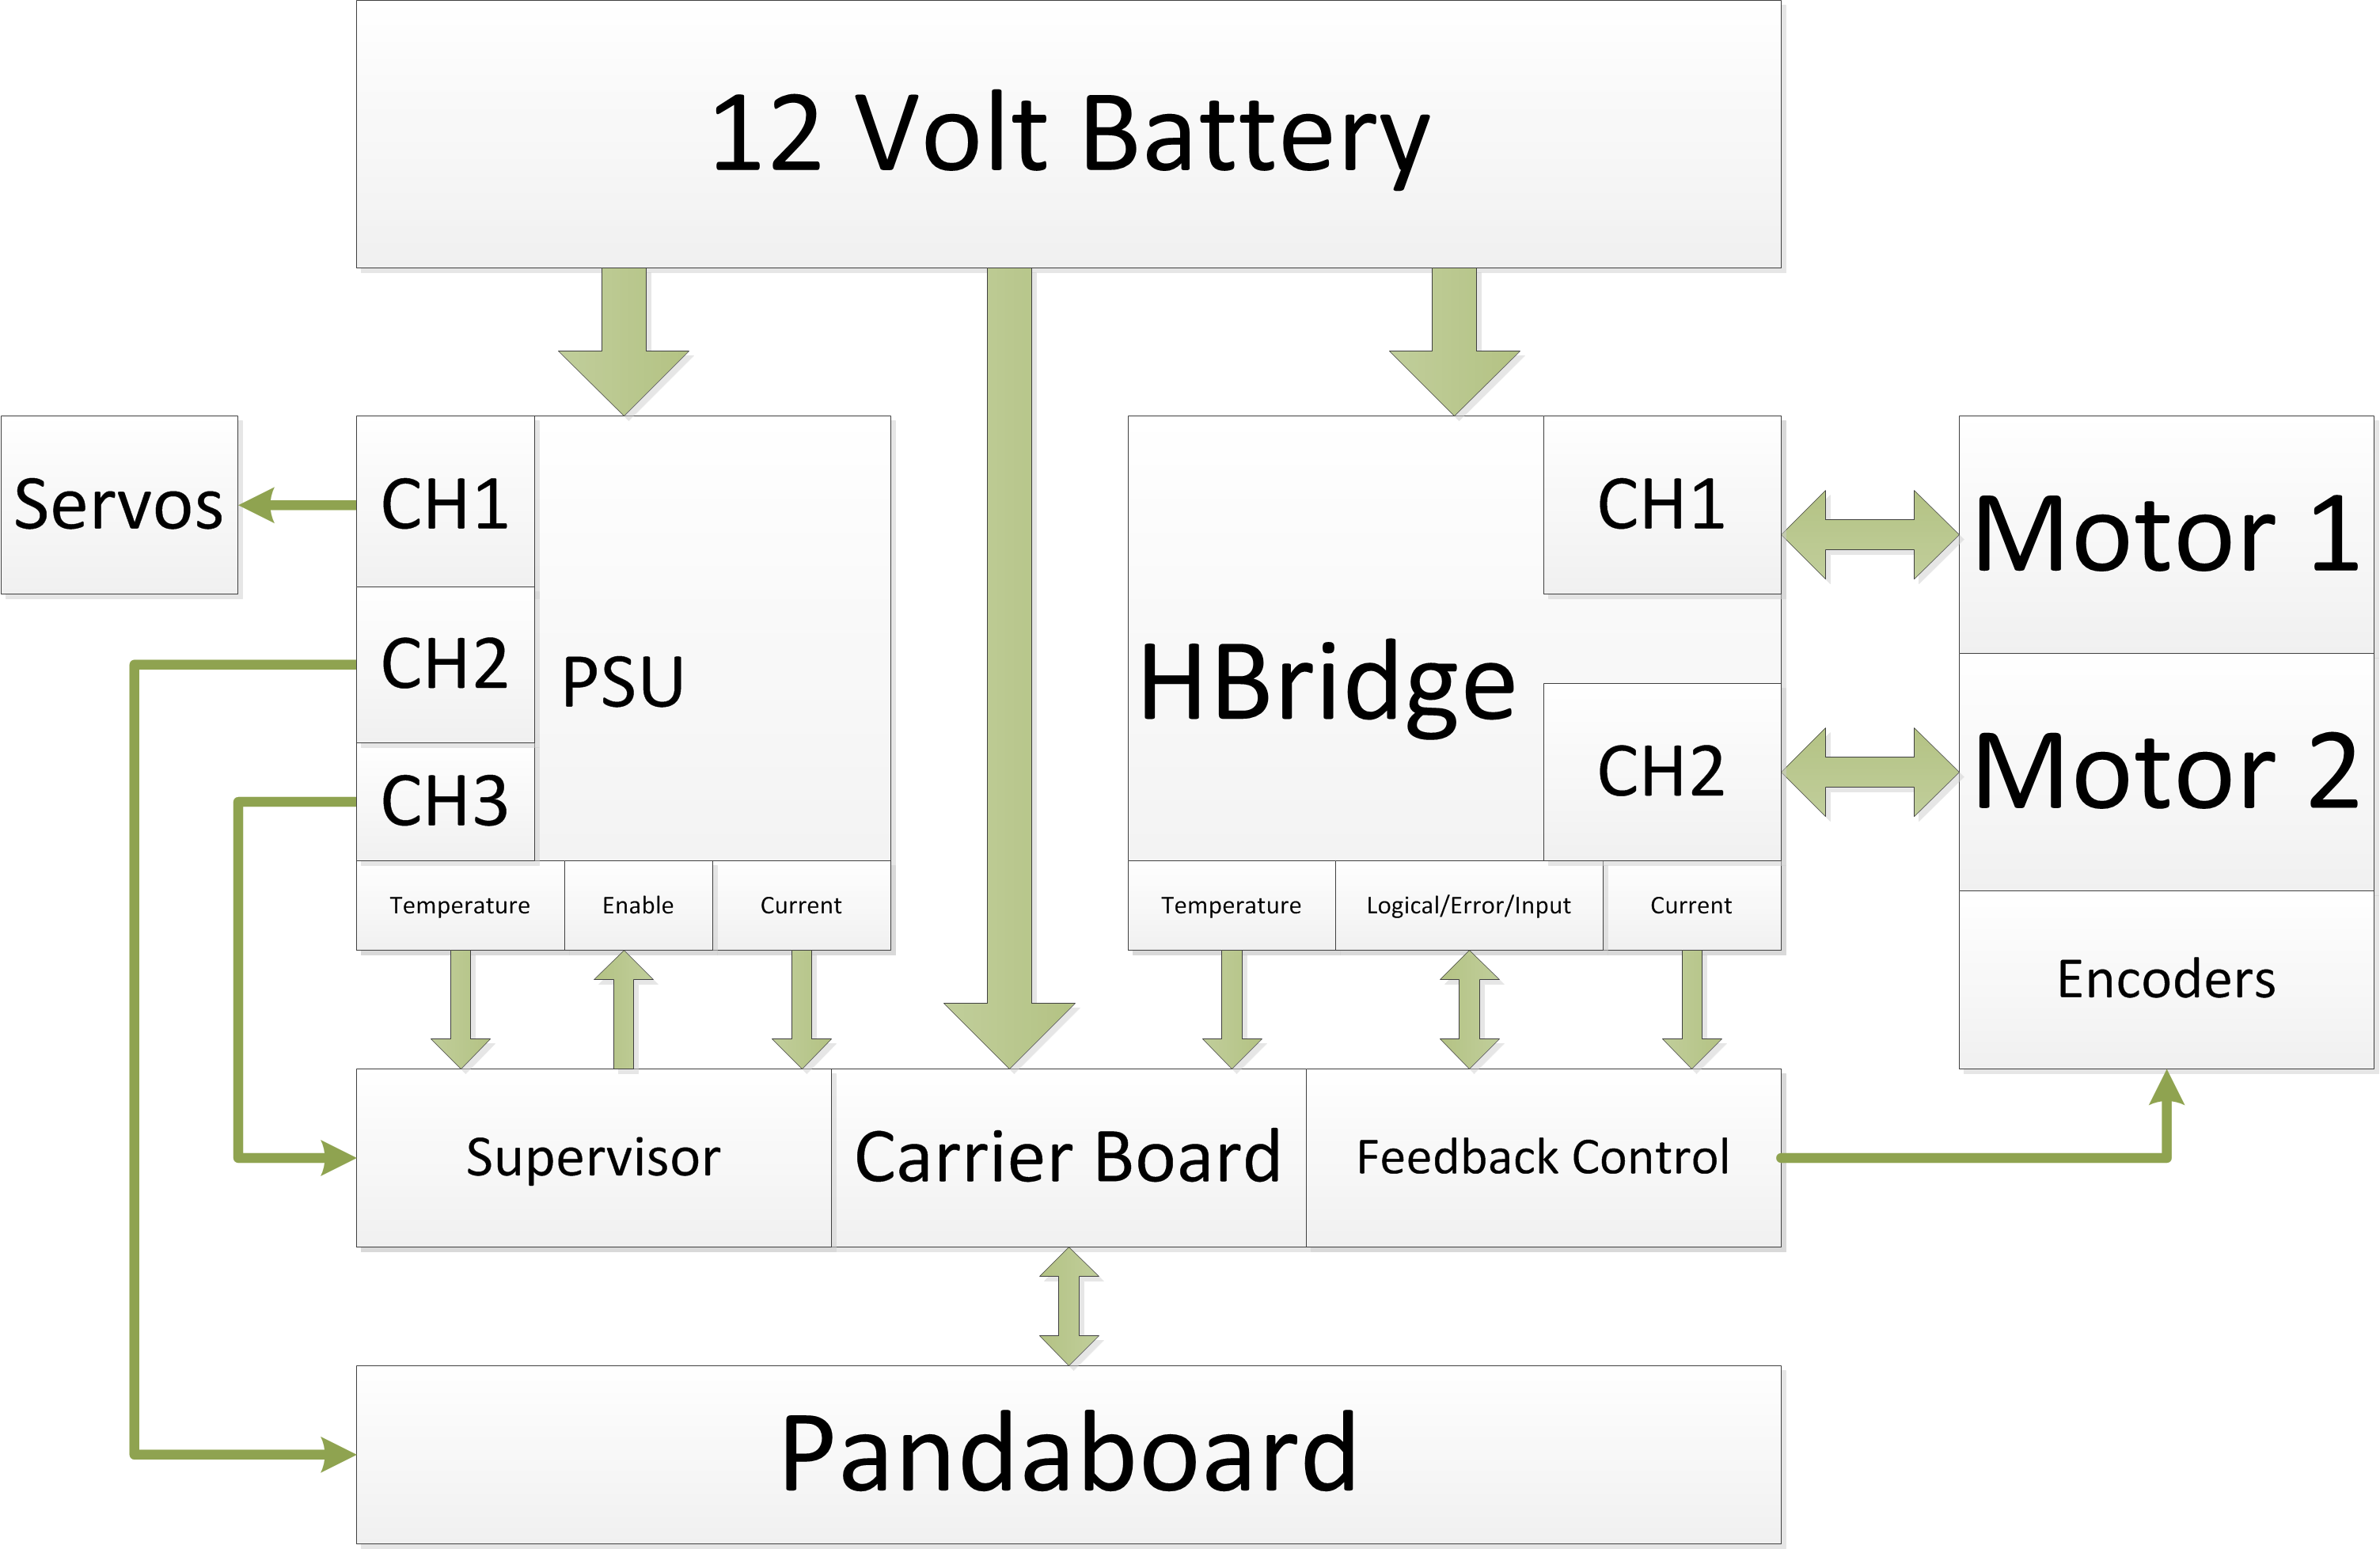
\includegraphics[width=6in]{Block_Diagram.png}
\caption{Block Diagram}
\end{figure}

 \end{document}
